\section{Sistema A – Controlo de Iluminação Interior}


\begin{figure}[H]
    \centering
    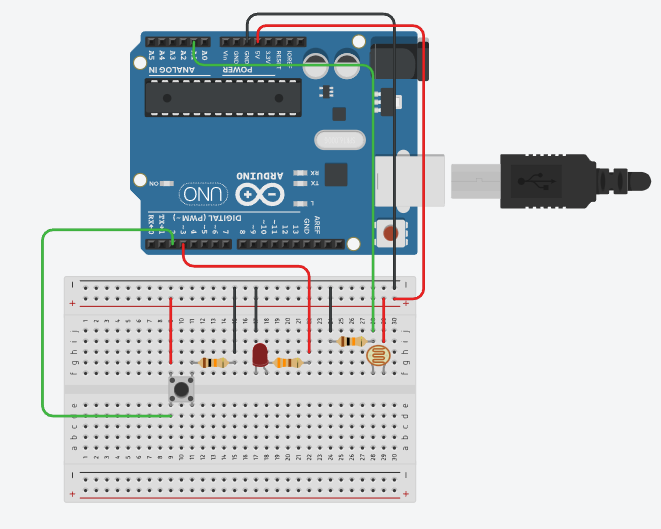
\includegraphics[scale=0.6]{images/hardware/sisA_tinkercad.png}
    \selectlanguage{portuguese}\caption{Esquema do Sistema A}
\end{figure}

\begin{figure}[H]
\centering
\setlength{\arrayrulewidth}{0.5mm}
\renewcommand{\arraystretch}{1.5}
\begin{tabular}{|l | c|} 
 \hline
 \multicolumn{1}{|c|}{Componentes} & \multicolumn{1}{|c|}{Quantidade}\\ [0.8ex] 
 \hline
 Fotorresistor & 1x \\ 
 \hline
 Botão & 1x \\
 \hline
 Arduino & 1x \\
 \hline
 Breadboard & 1x\\
 \hline
 LED & 1x\\
 \hline
 Resistência 330 Ohm & 1x\\
 \hline
 Resistência 10k Ohm & 2x  \\
 \hline
\end{tabular}
\selectlanguage{portuguese}\caption{Componentes Utilizados}
\end{figure}

A resistência de 330 Ohm encontra-se ligada ao LED.

As duas resistências de 10k Ohm encontram-se ligadas ao fotorresistor e ao botão.

O Arduino recebe o input do fotorresistor através do pino analógico A1.

O LED está ligado à porta nº 3 que serve como output.

O Arduino recebe o input do botão através da porta nº 2. O Botão serve de interrupt do sistema.

\begin{figure}[H]
    \centering
    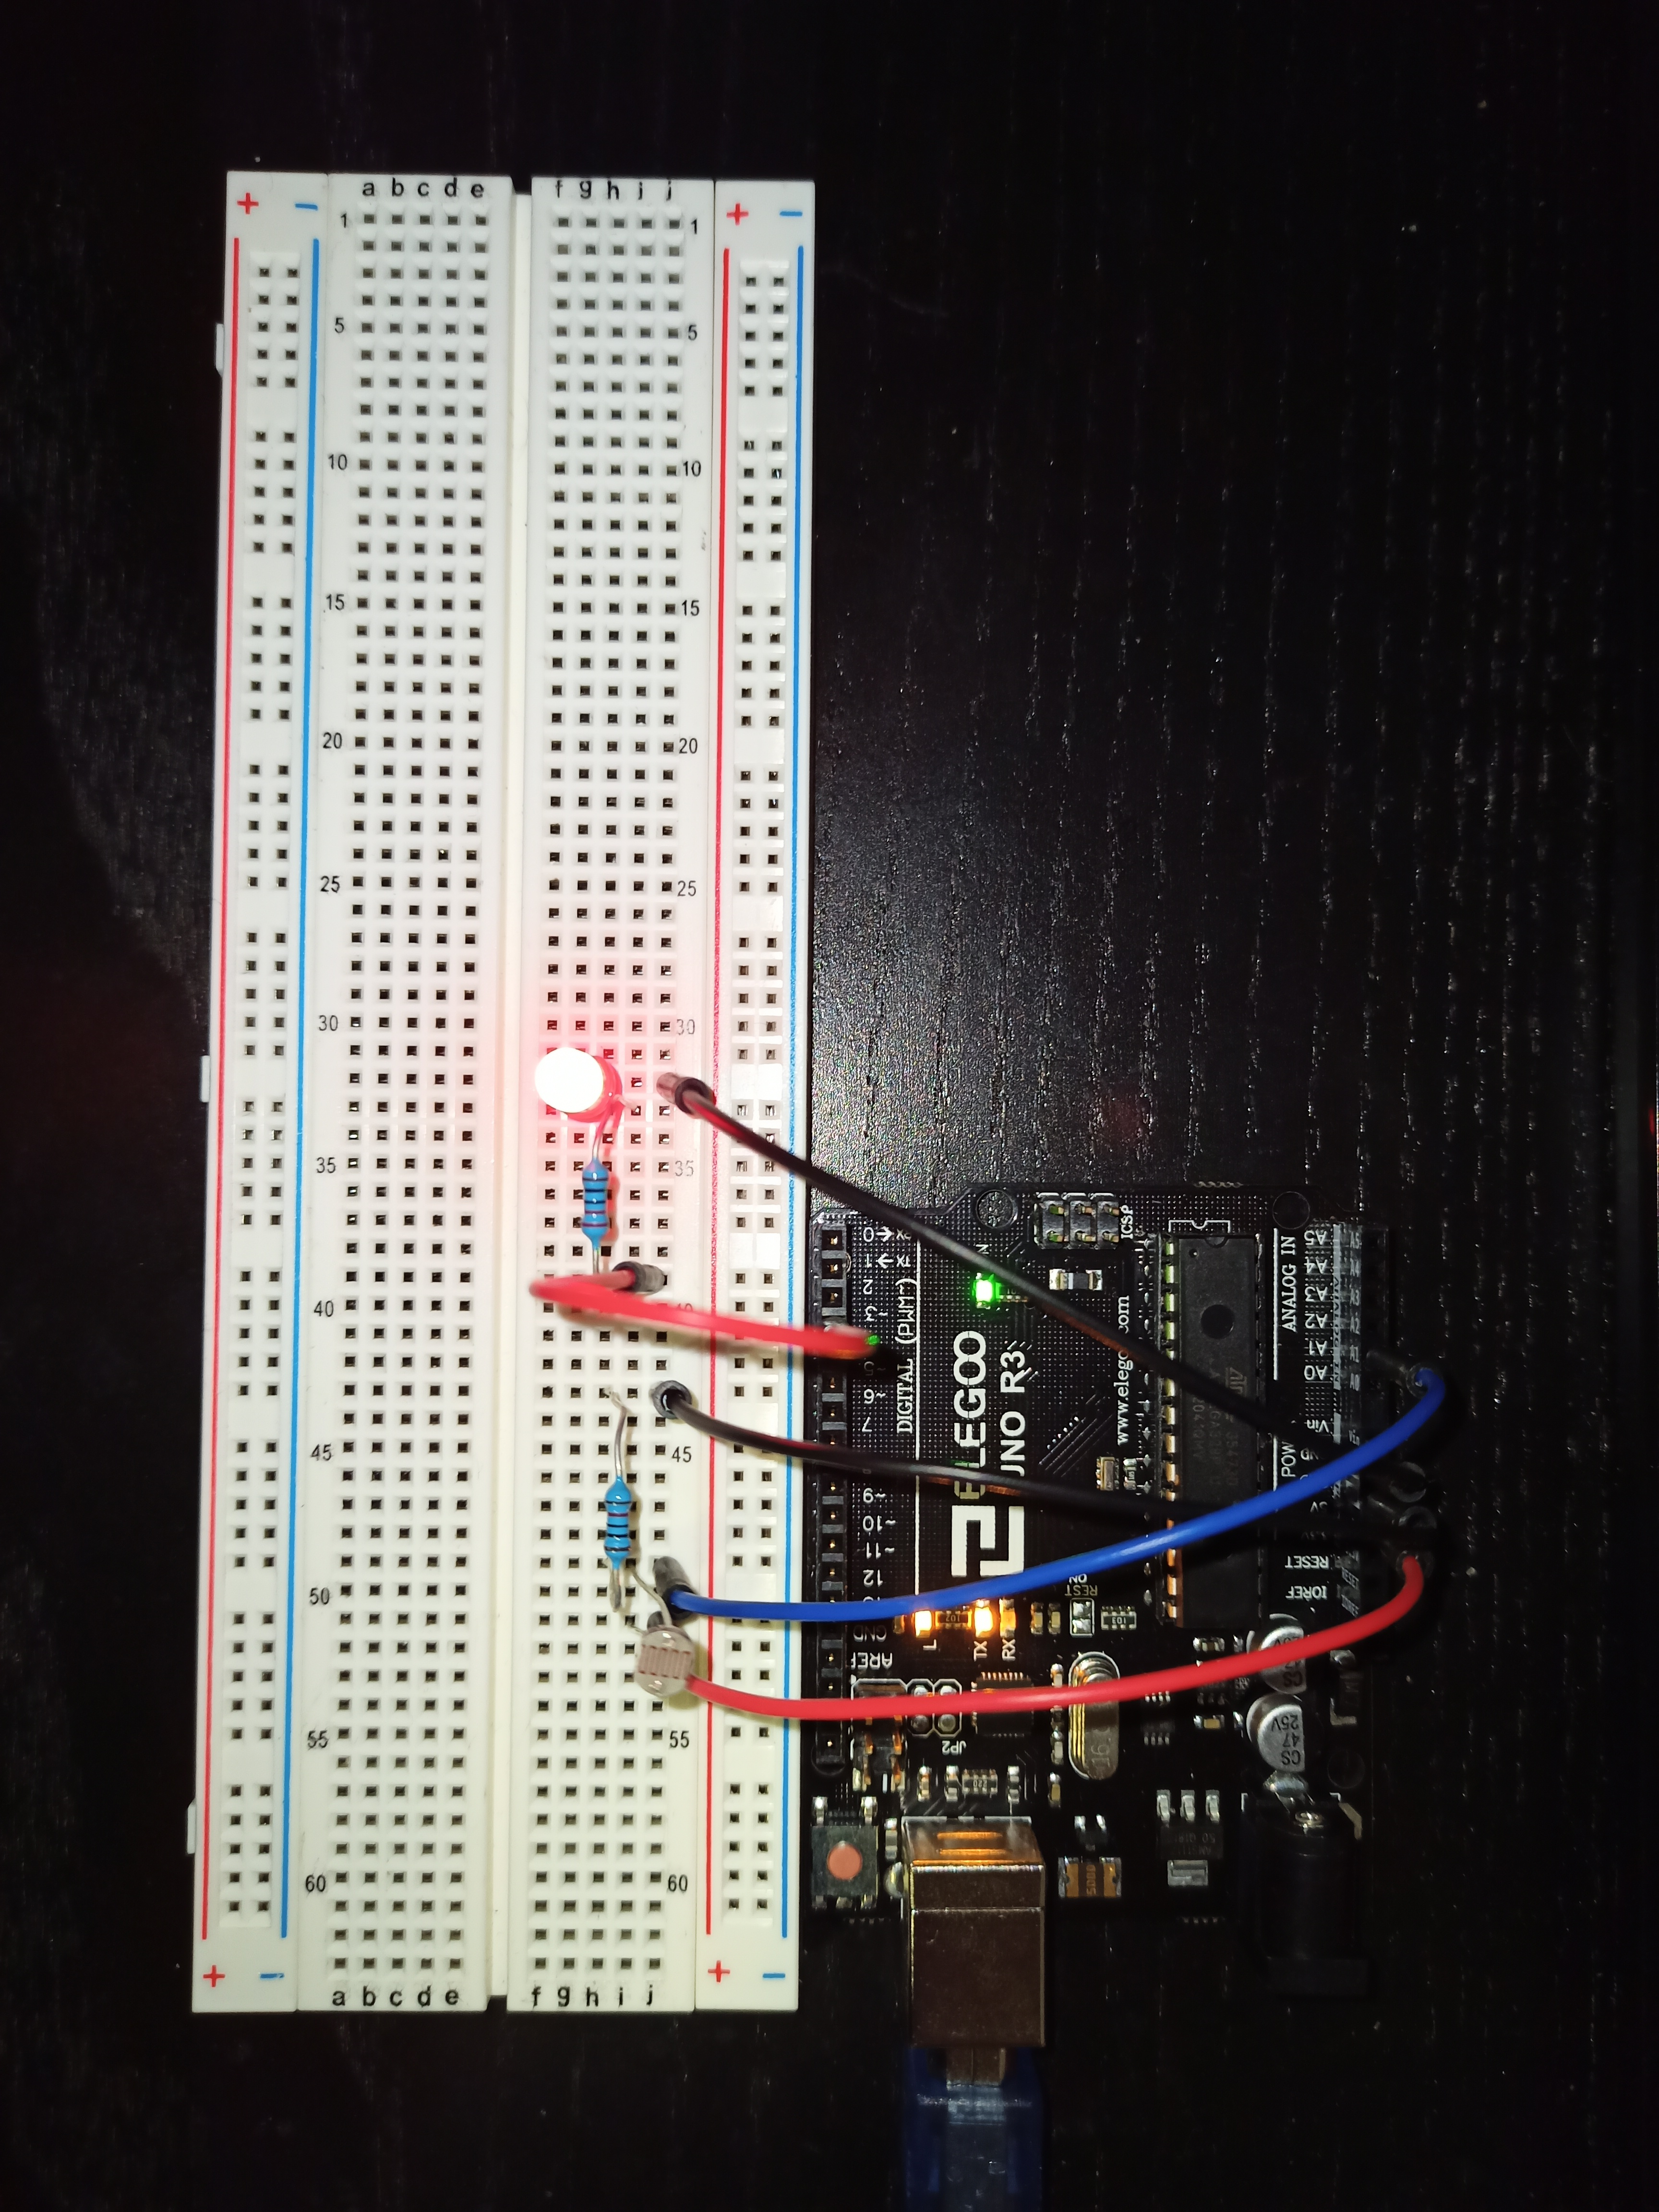
\includegraphics[scale=0.05,angle=90]{images/hardware/sisA_IRL.jpg}
    \selectlanguage{portuguese}\caption{Esquema montado do Sistema A}
\end{figure}